\documentclass[../DefinizioneDiProdotto.tex]{subfiles}
\begin{document}

\begin{appendices}

\section{Diagrammi riassuntivi package significativi}
	Di seguito sono riportati tutti i package dell'applicativo ad eccezione della \verb|view|, essendo applicato il pattern MVP, per chiarire la relazione tra le componenti e le classi al suo interno. Per chiarezza ed esigenza di spazio le classi rappresentate all'interno dei package sono senza metodi e attributi.

		\begin{figure}[H]
			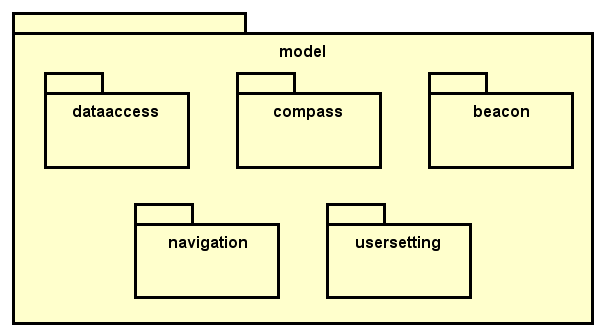
\includegraphics[angle=90,width=\textwidth, height=\textheight, keepaspectratio]{diagrams/ModelCompleteNoMethods/PNGpackage/model}
			\label{modelPackage}
			\caption{Diagramma delle classi - model}
		\end{figure}
	
		\begin{figure}[H]
			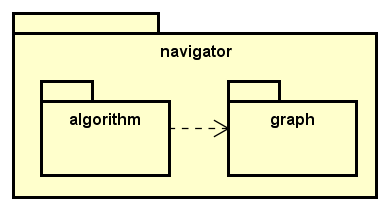
\includegraphics[angle=90,width=\textwidth,, height=580pt, keepaspectratio]{diagrams/ModelCompleteNoMethods/PNGpackage/navigator}
			\label{navigatorPackage}
			\caption{Diagramma delle classi - model::navigator}
		\end{figure}
	
		\begin{figure}[H]
			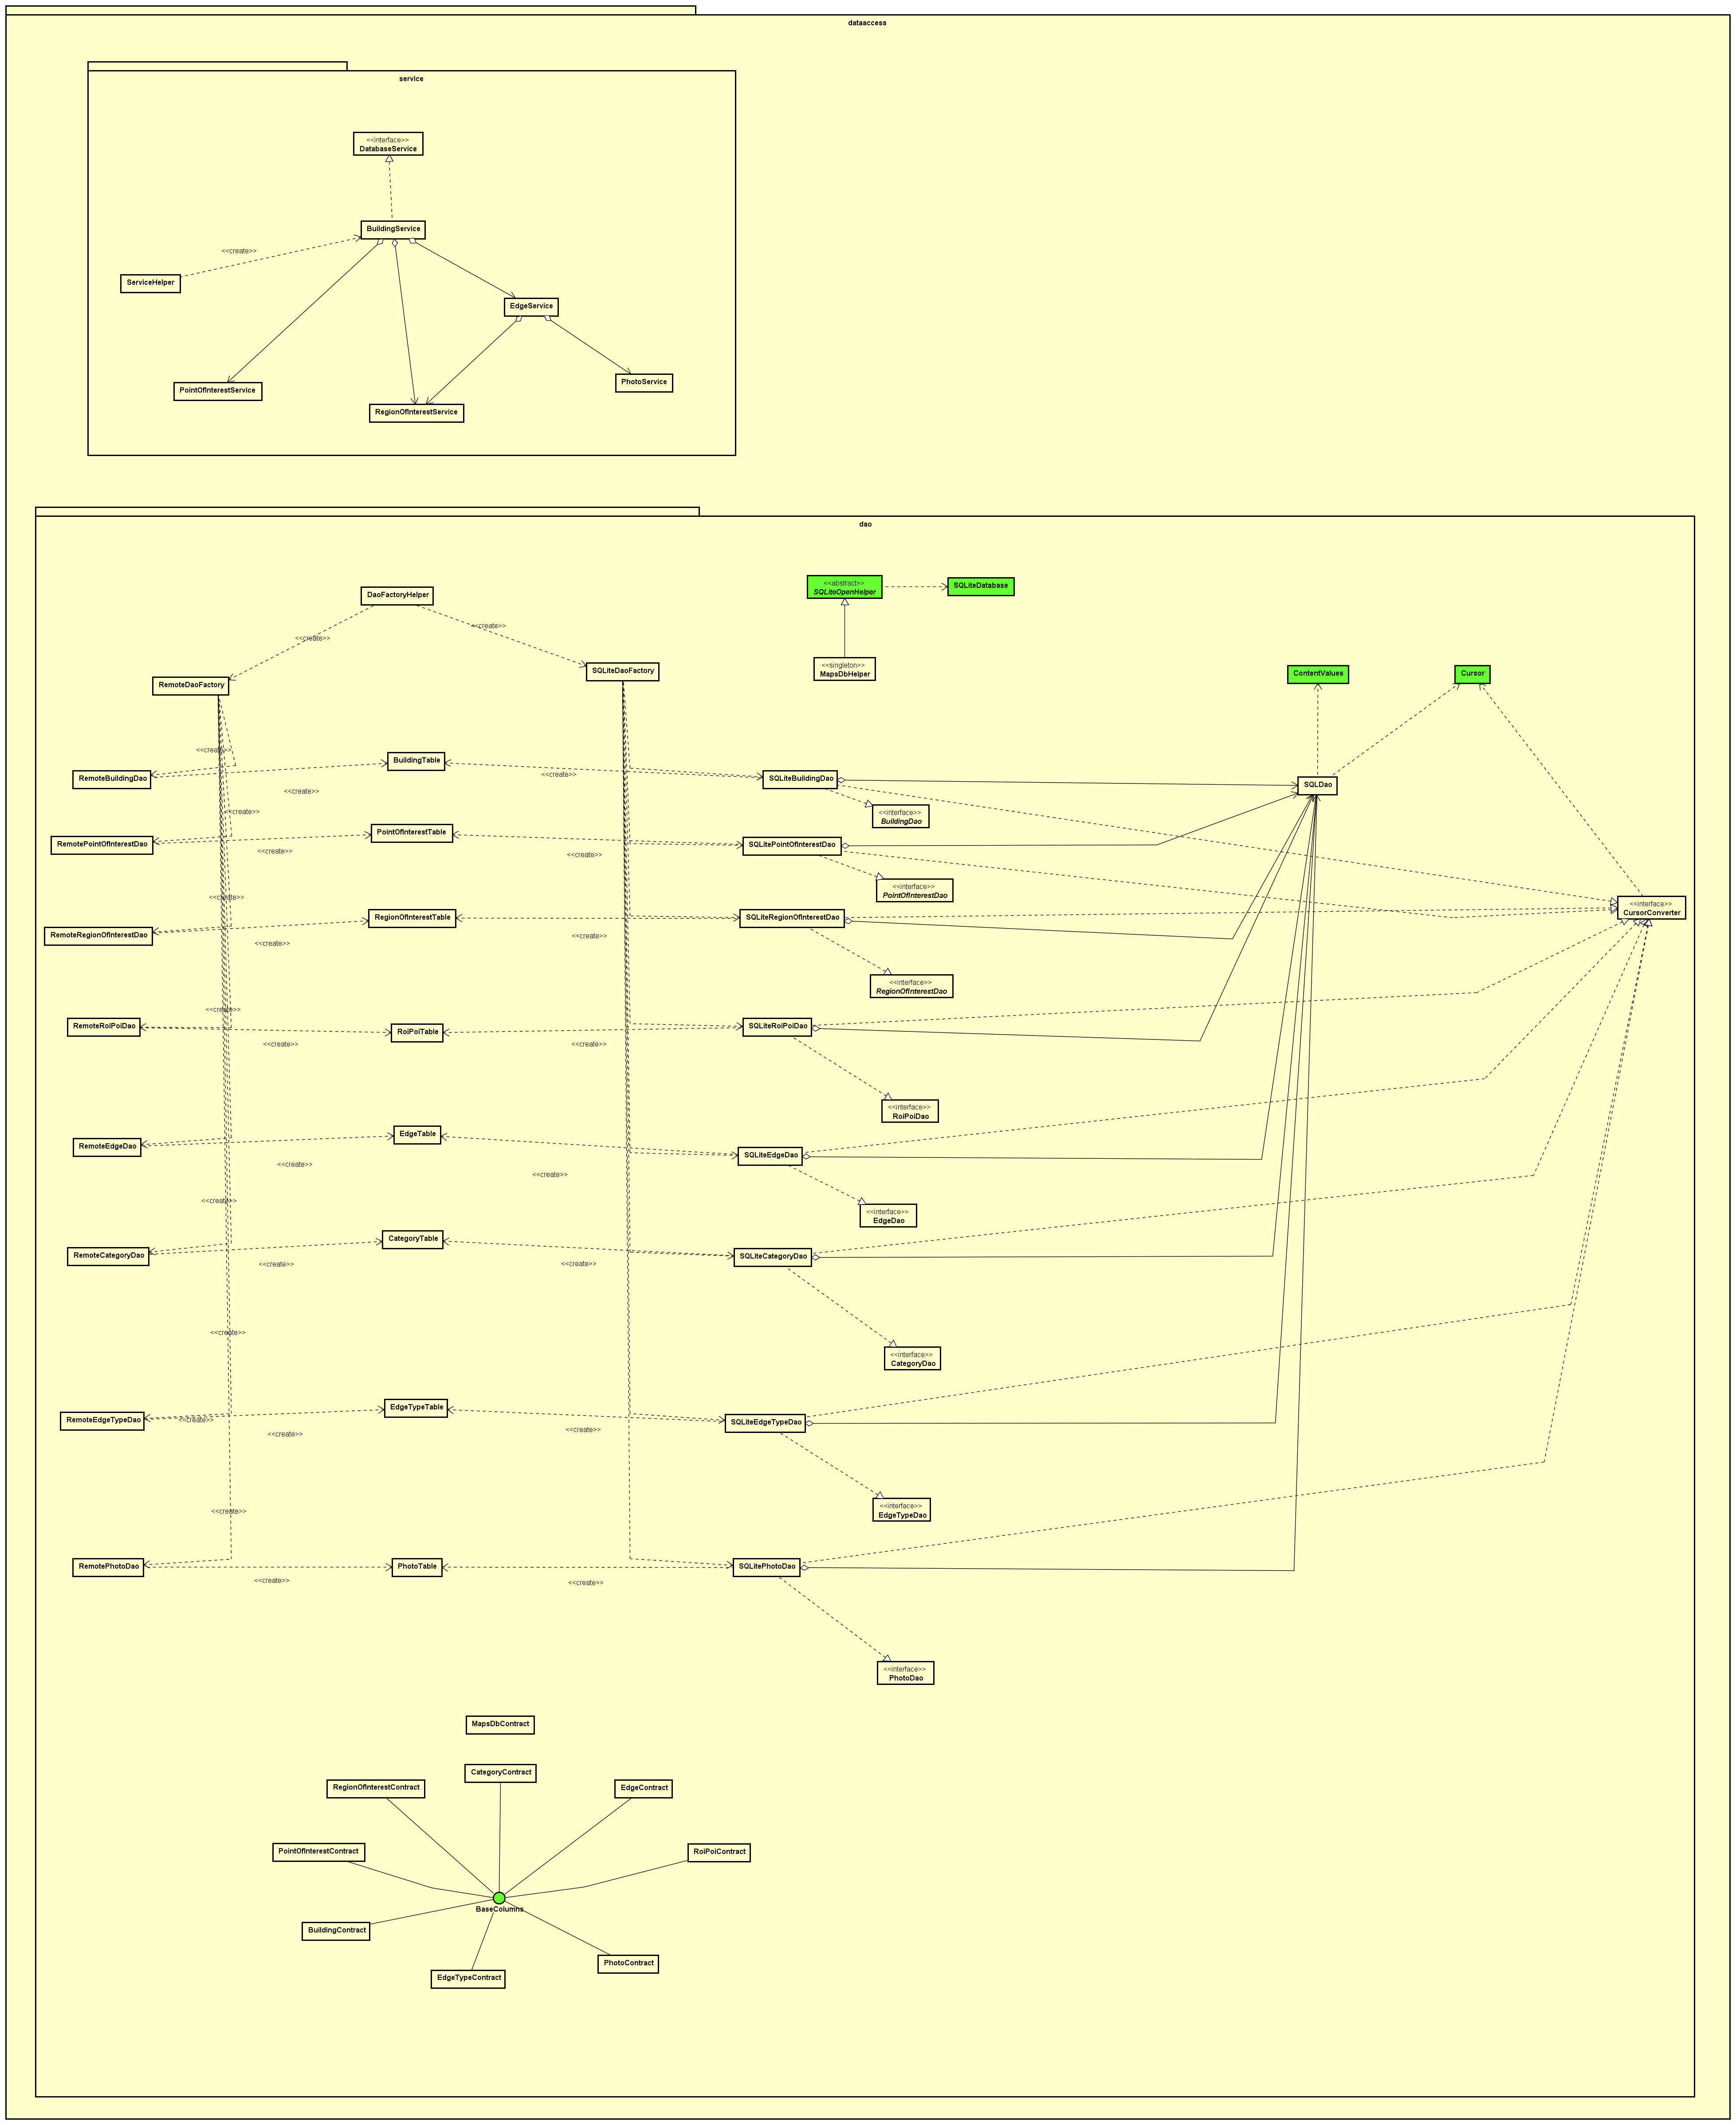
\includegraphics[width=\textwidth]{diagrams/ModelCompleteNoMethods/PNGpackage/dataaccess}
			\label{dataaccessPackage}
			\caption{Diagramma delle classi - model::dataaccess}
		\end{figure}
		
		\begin{figure}[H]
			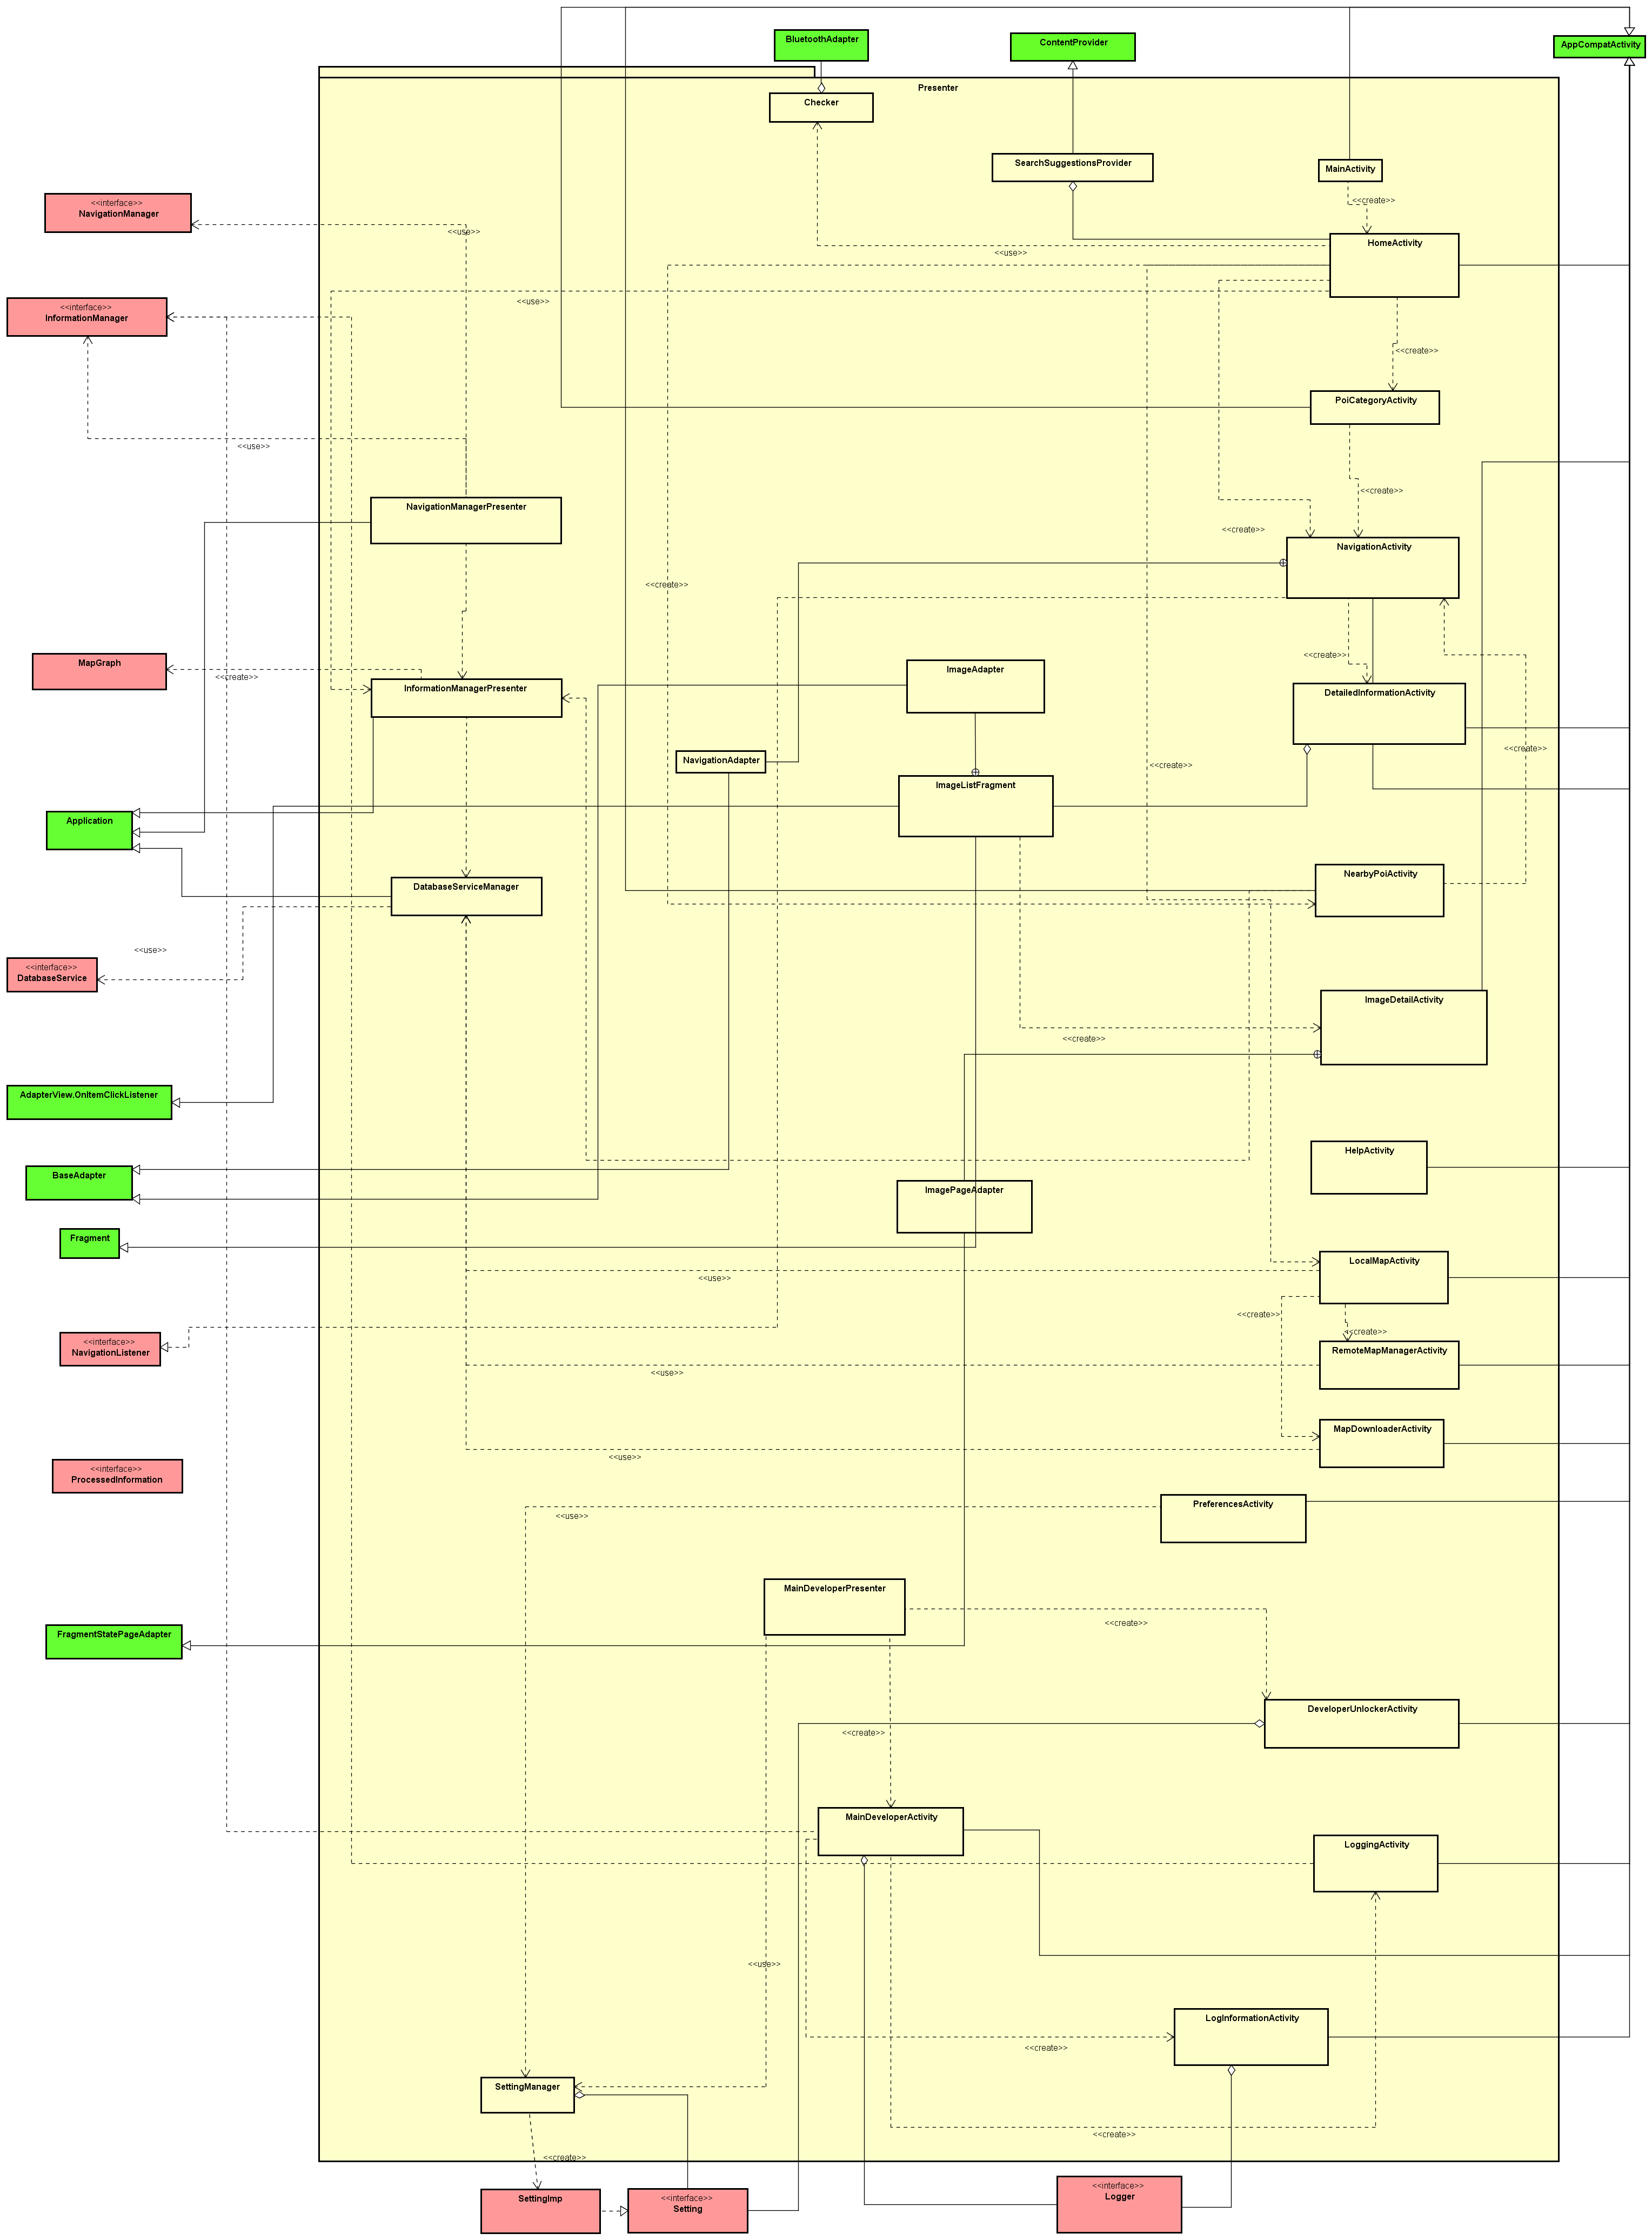
\includegraphics[width=\textwidth]{diagrams/ModelCompleteNoMethods/PNGpackage/presenter}
			\label{presenterPackage}
			\caption{Diagramma delle classi - presenter}
		\end{figure}

		%\begin{figure}[H]
			%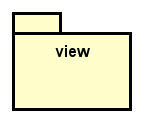
\includegraphics[scale=0.5]{diagrams/ModelCompleteNoMethods/PNGpackage/view}
			%\label{modelPackage}
			%\caption{Diagramma delle classi - view}
		%\end{figure}

\end{appendices}

\end{document}